\chapter{Travail réalisé}
    \section{Présentation des outils}
        \subsection{Raspberry Pi}
        Le \textit{Raspberry Pi} est un ordinateur portable de petite taille, doté d'un processeur ARM et d'un système d'exploitation Linux.
        \begin{figure}[h]
            \centering
            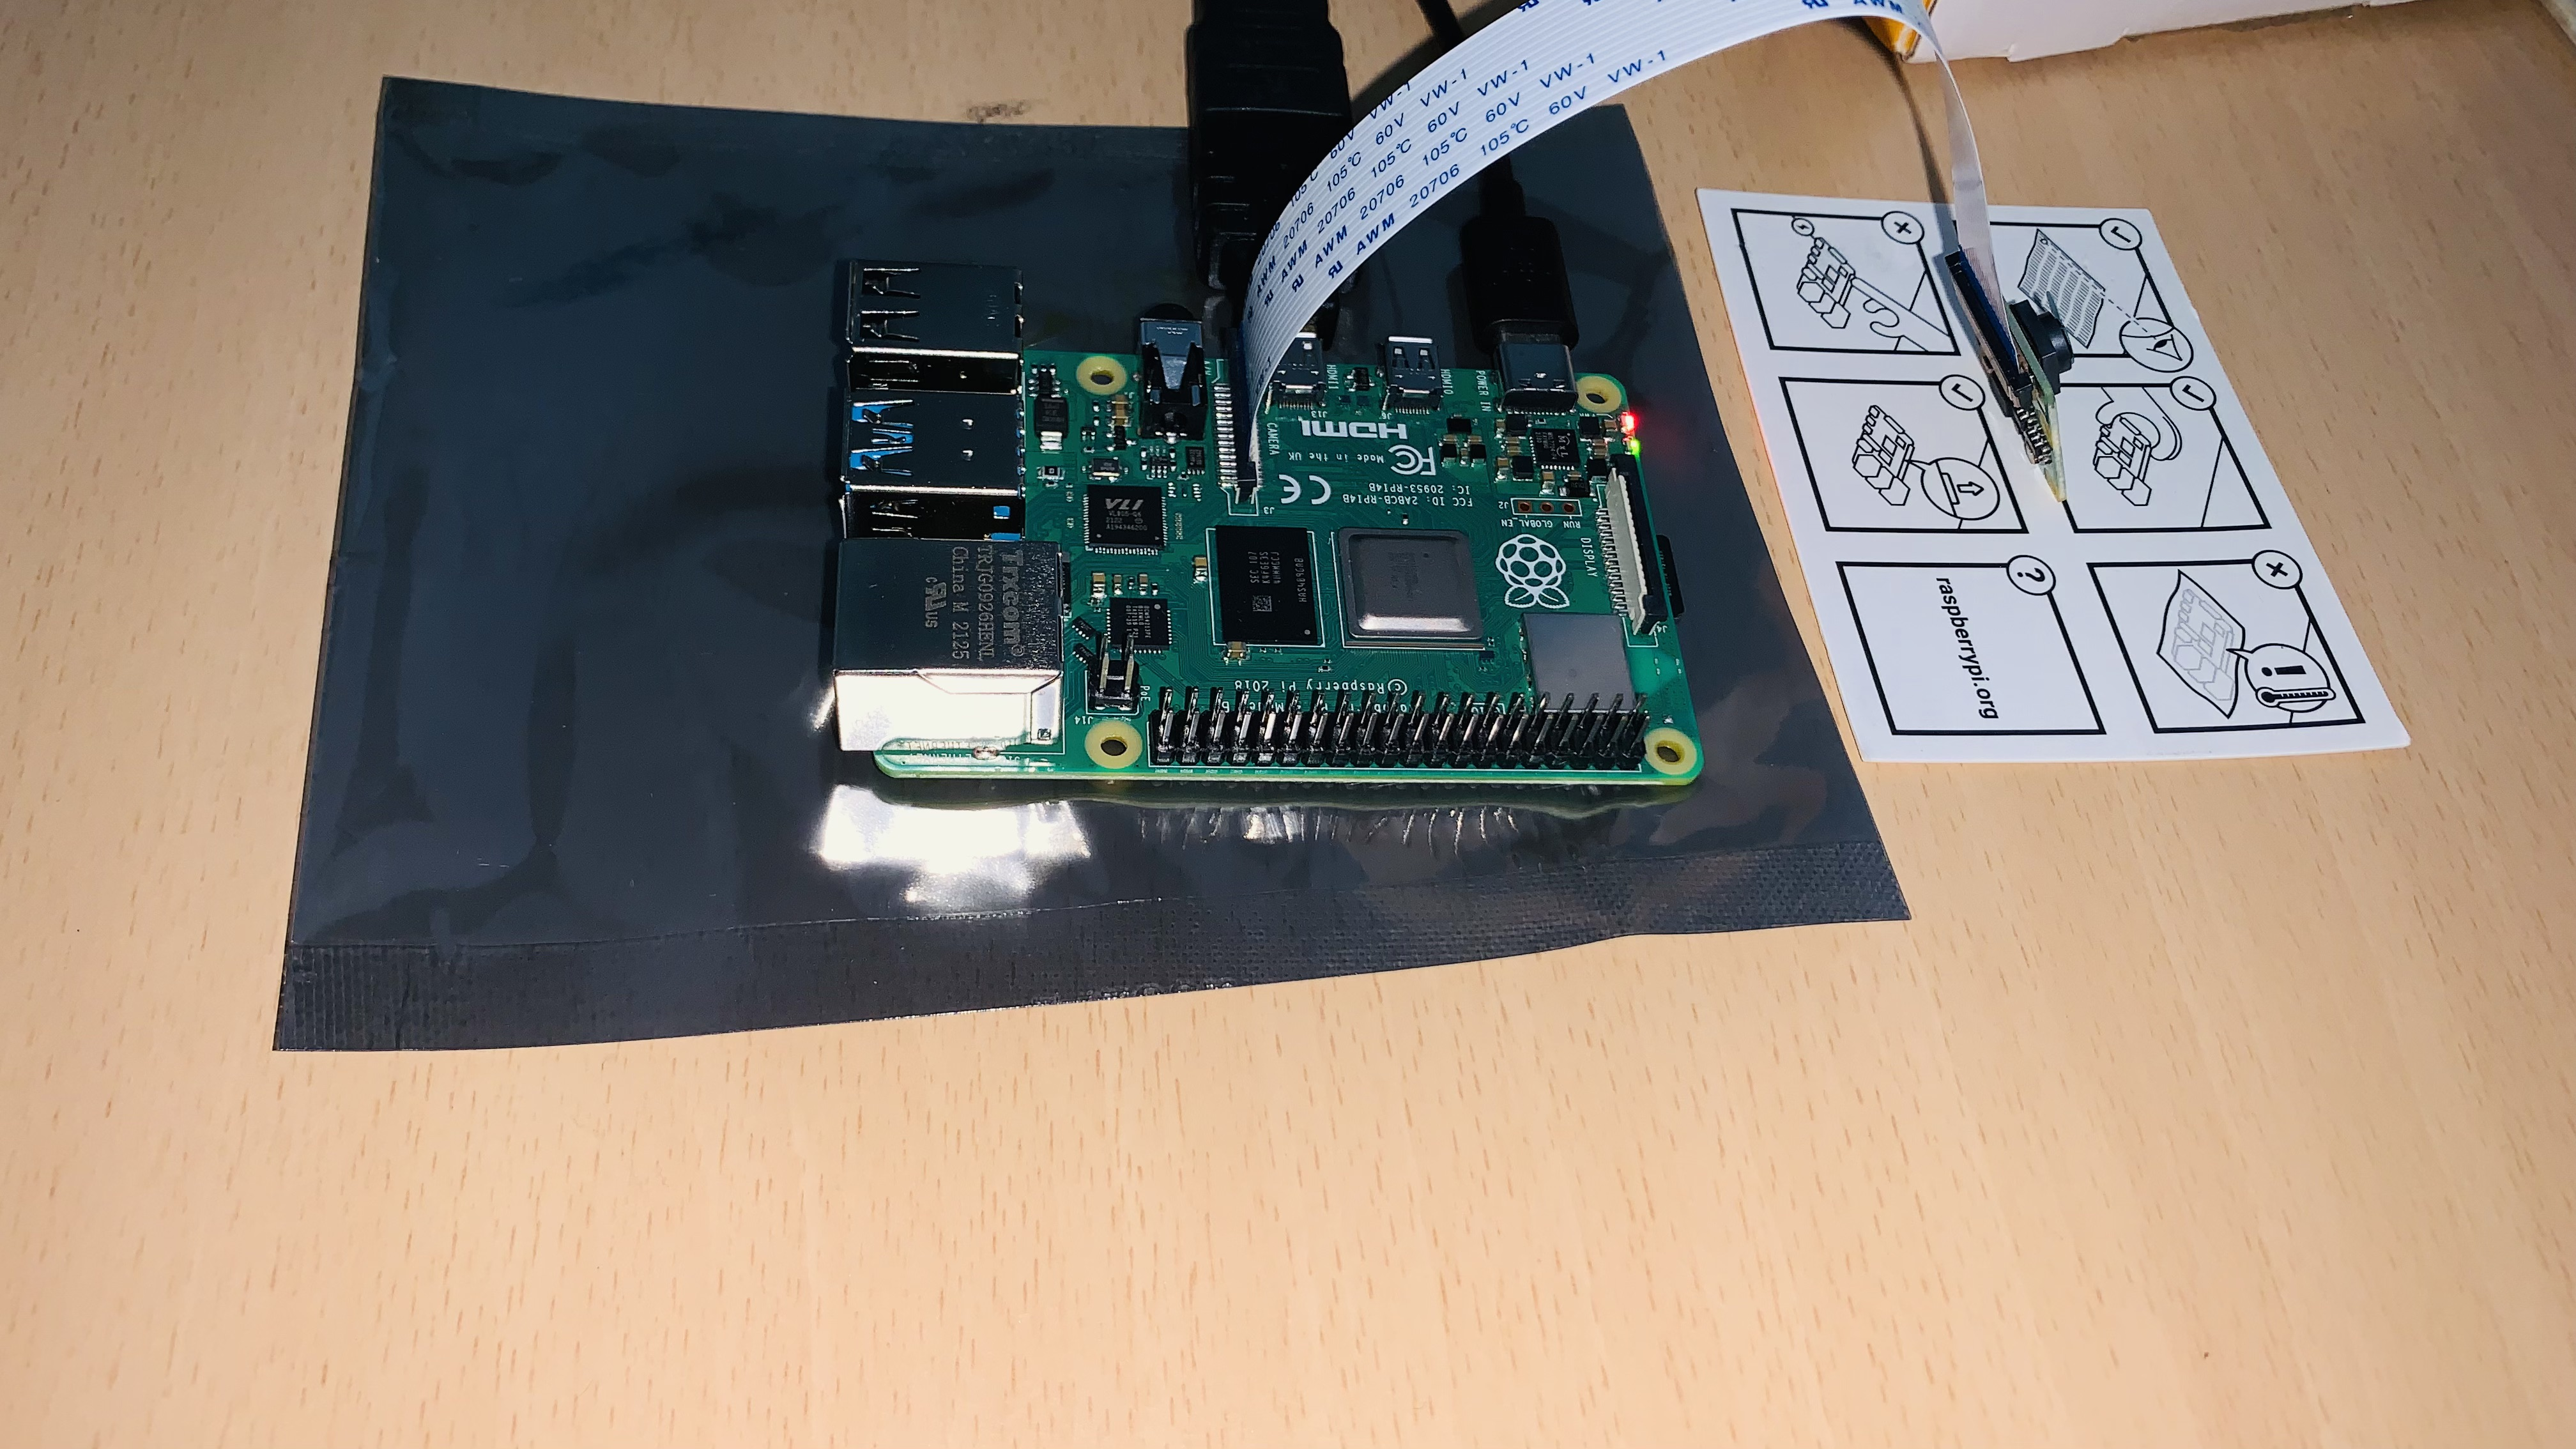
\includegraphics[scale=0.03]{raspberry_pi.jpeg}
            \caption{Raspberry Pi 4}
        \end{figure}

        \subsection{Module de capture vidéo (Raspberry Pi) V2}
        Le module de capture vidéo (Raspberry Pi) V2 est un module de captation vidéo qui permet de capturer des images et des vidéos.
        \begin{figure}[h]
            \centering        
            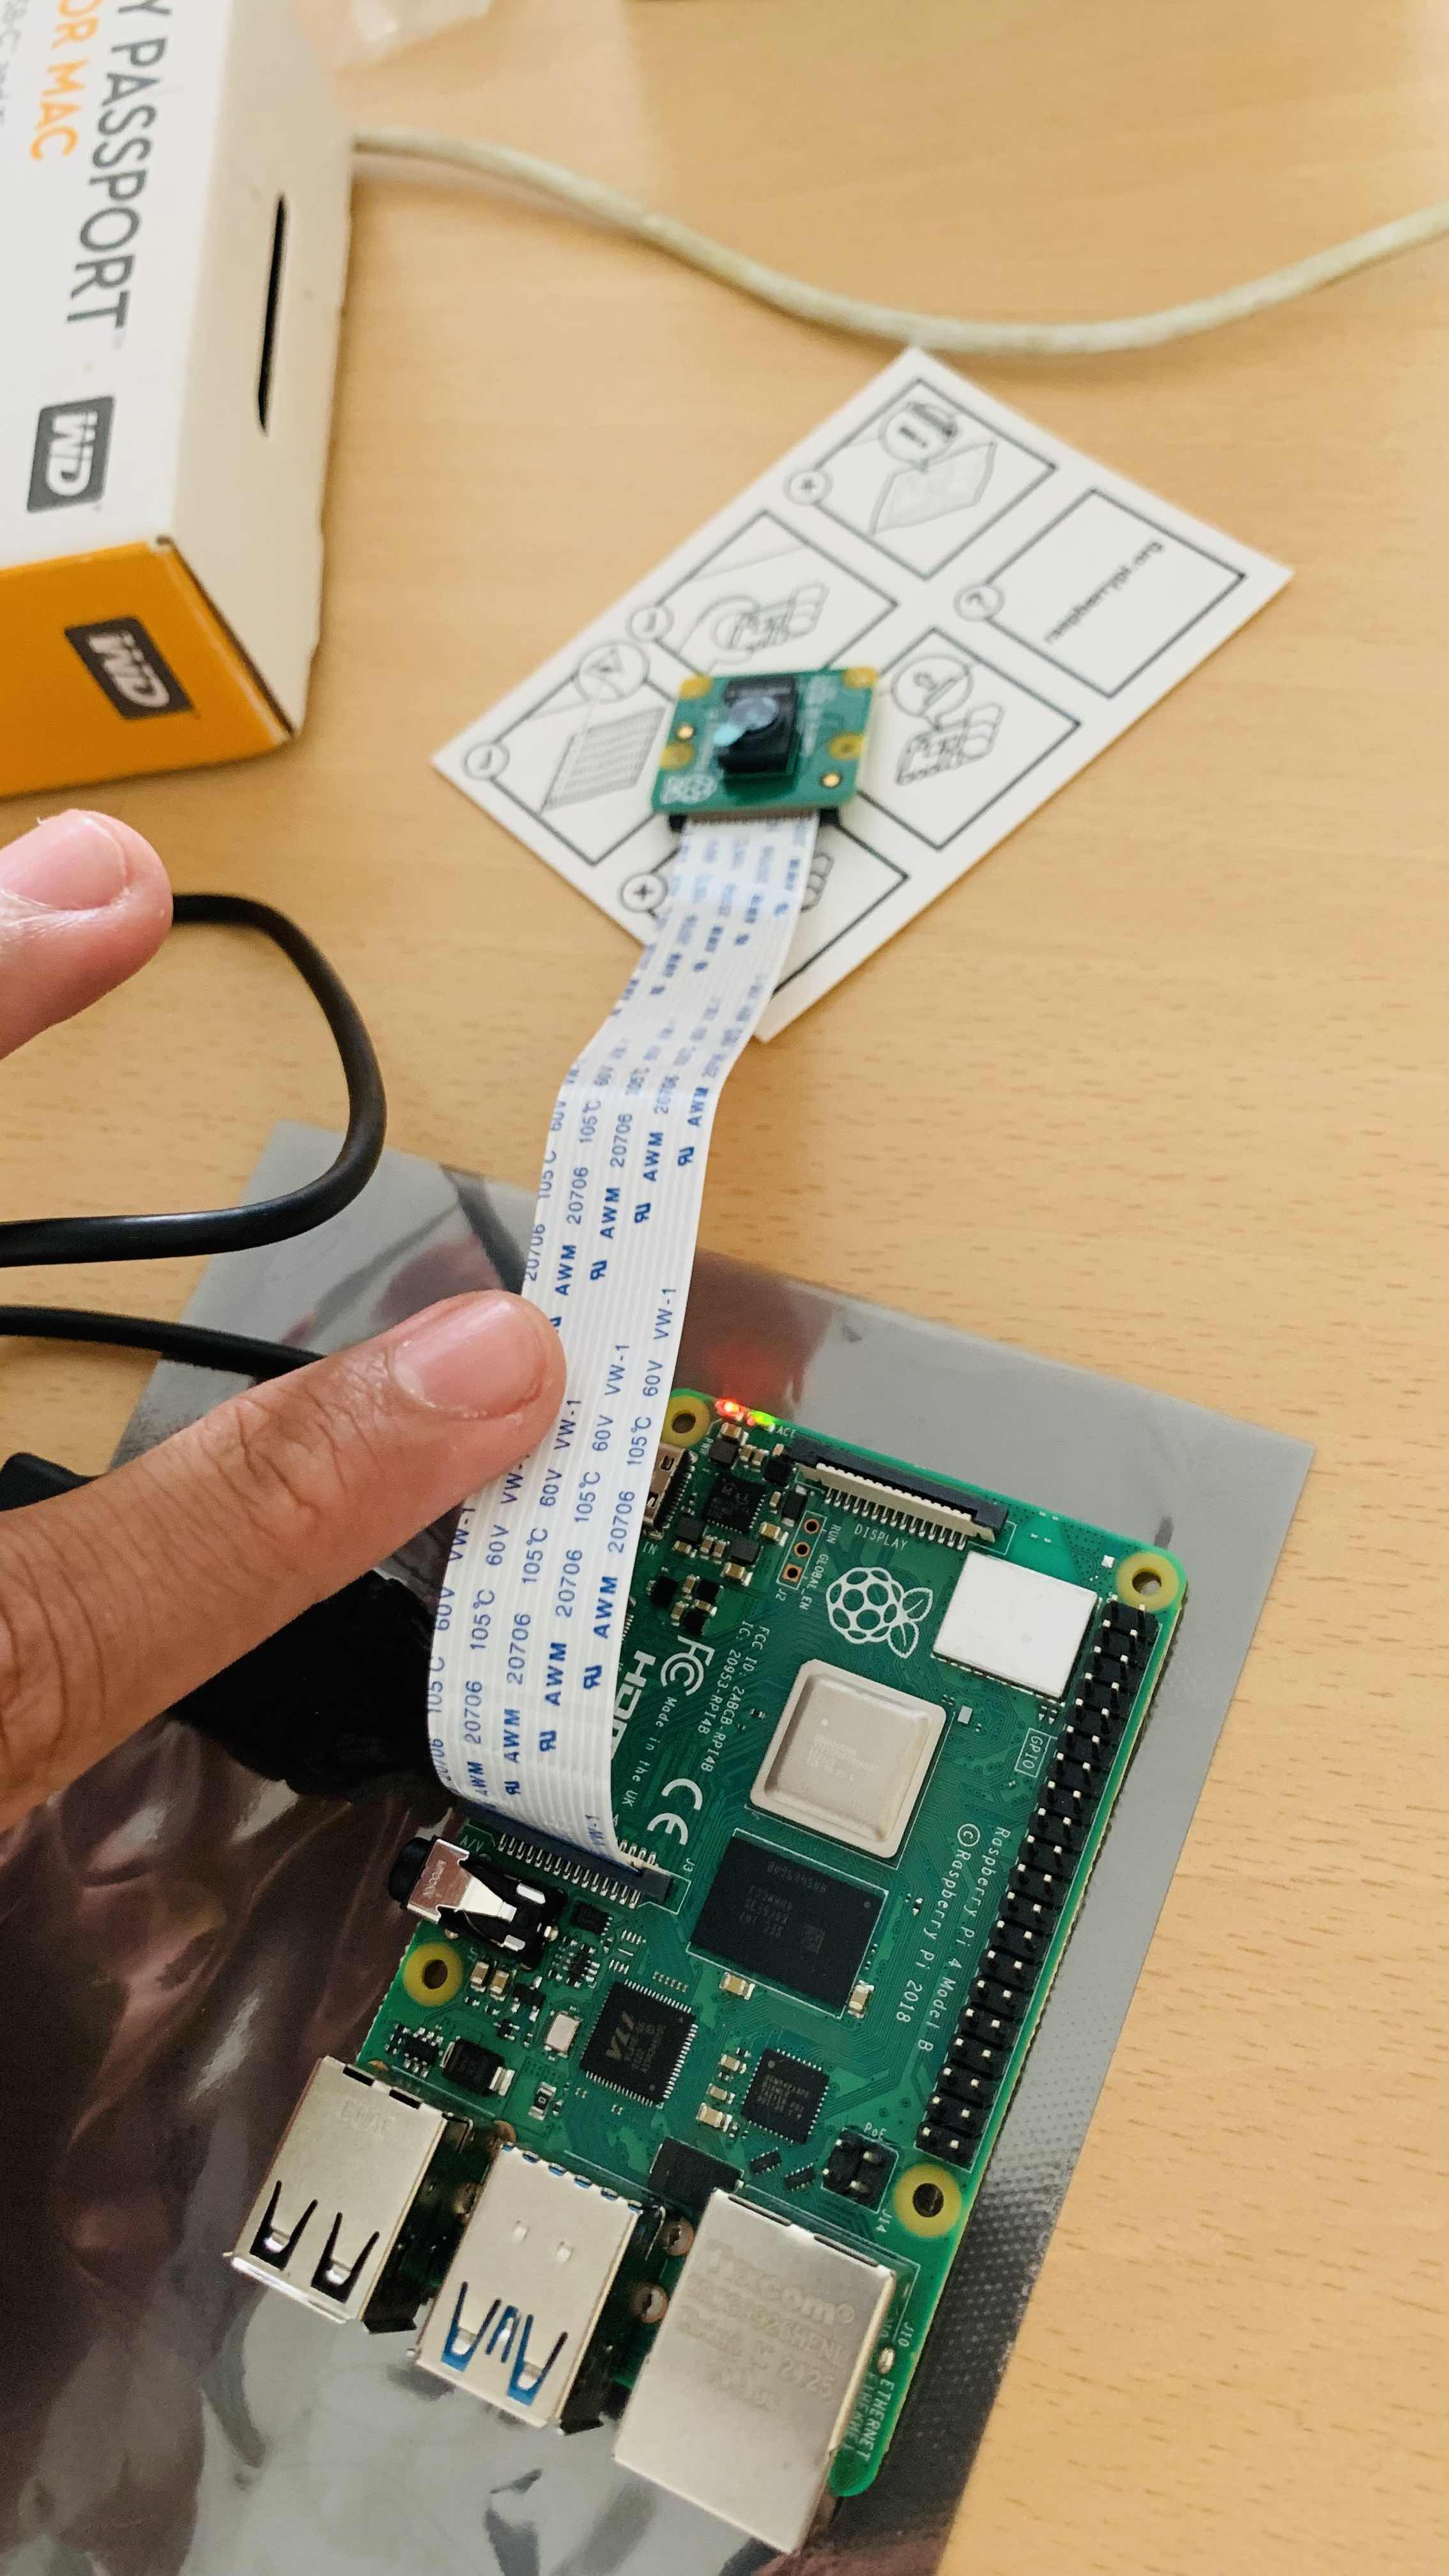
\includegraphics[scale=0.03]{module_camera_v2.jpeg}
            \caption{Module de capture vidéo (Raspberry Pi) V2}
        \end{figure}

        \vspace{0.5cm}
 
        \subsection{Ecran LCD (Raspberry Pi) tailles}
        Avec le \textit{Raspberry Pi} un écran LCD de 7 pouces  permettant de visualiser les images et les vidéos et d'interagir avec l'ordinateur grâce à son écran tactile. 
        \begin{figure}[h]
            \centering
            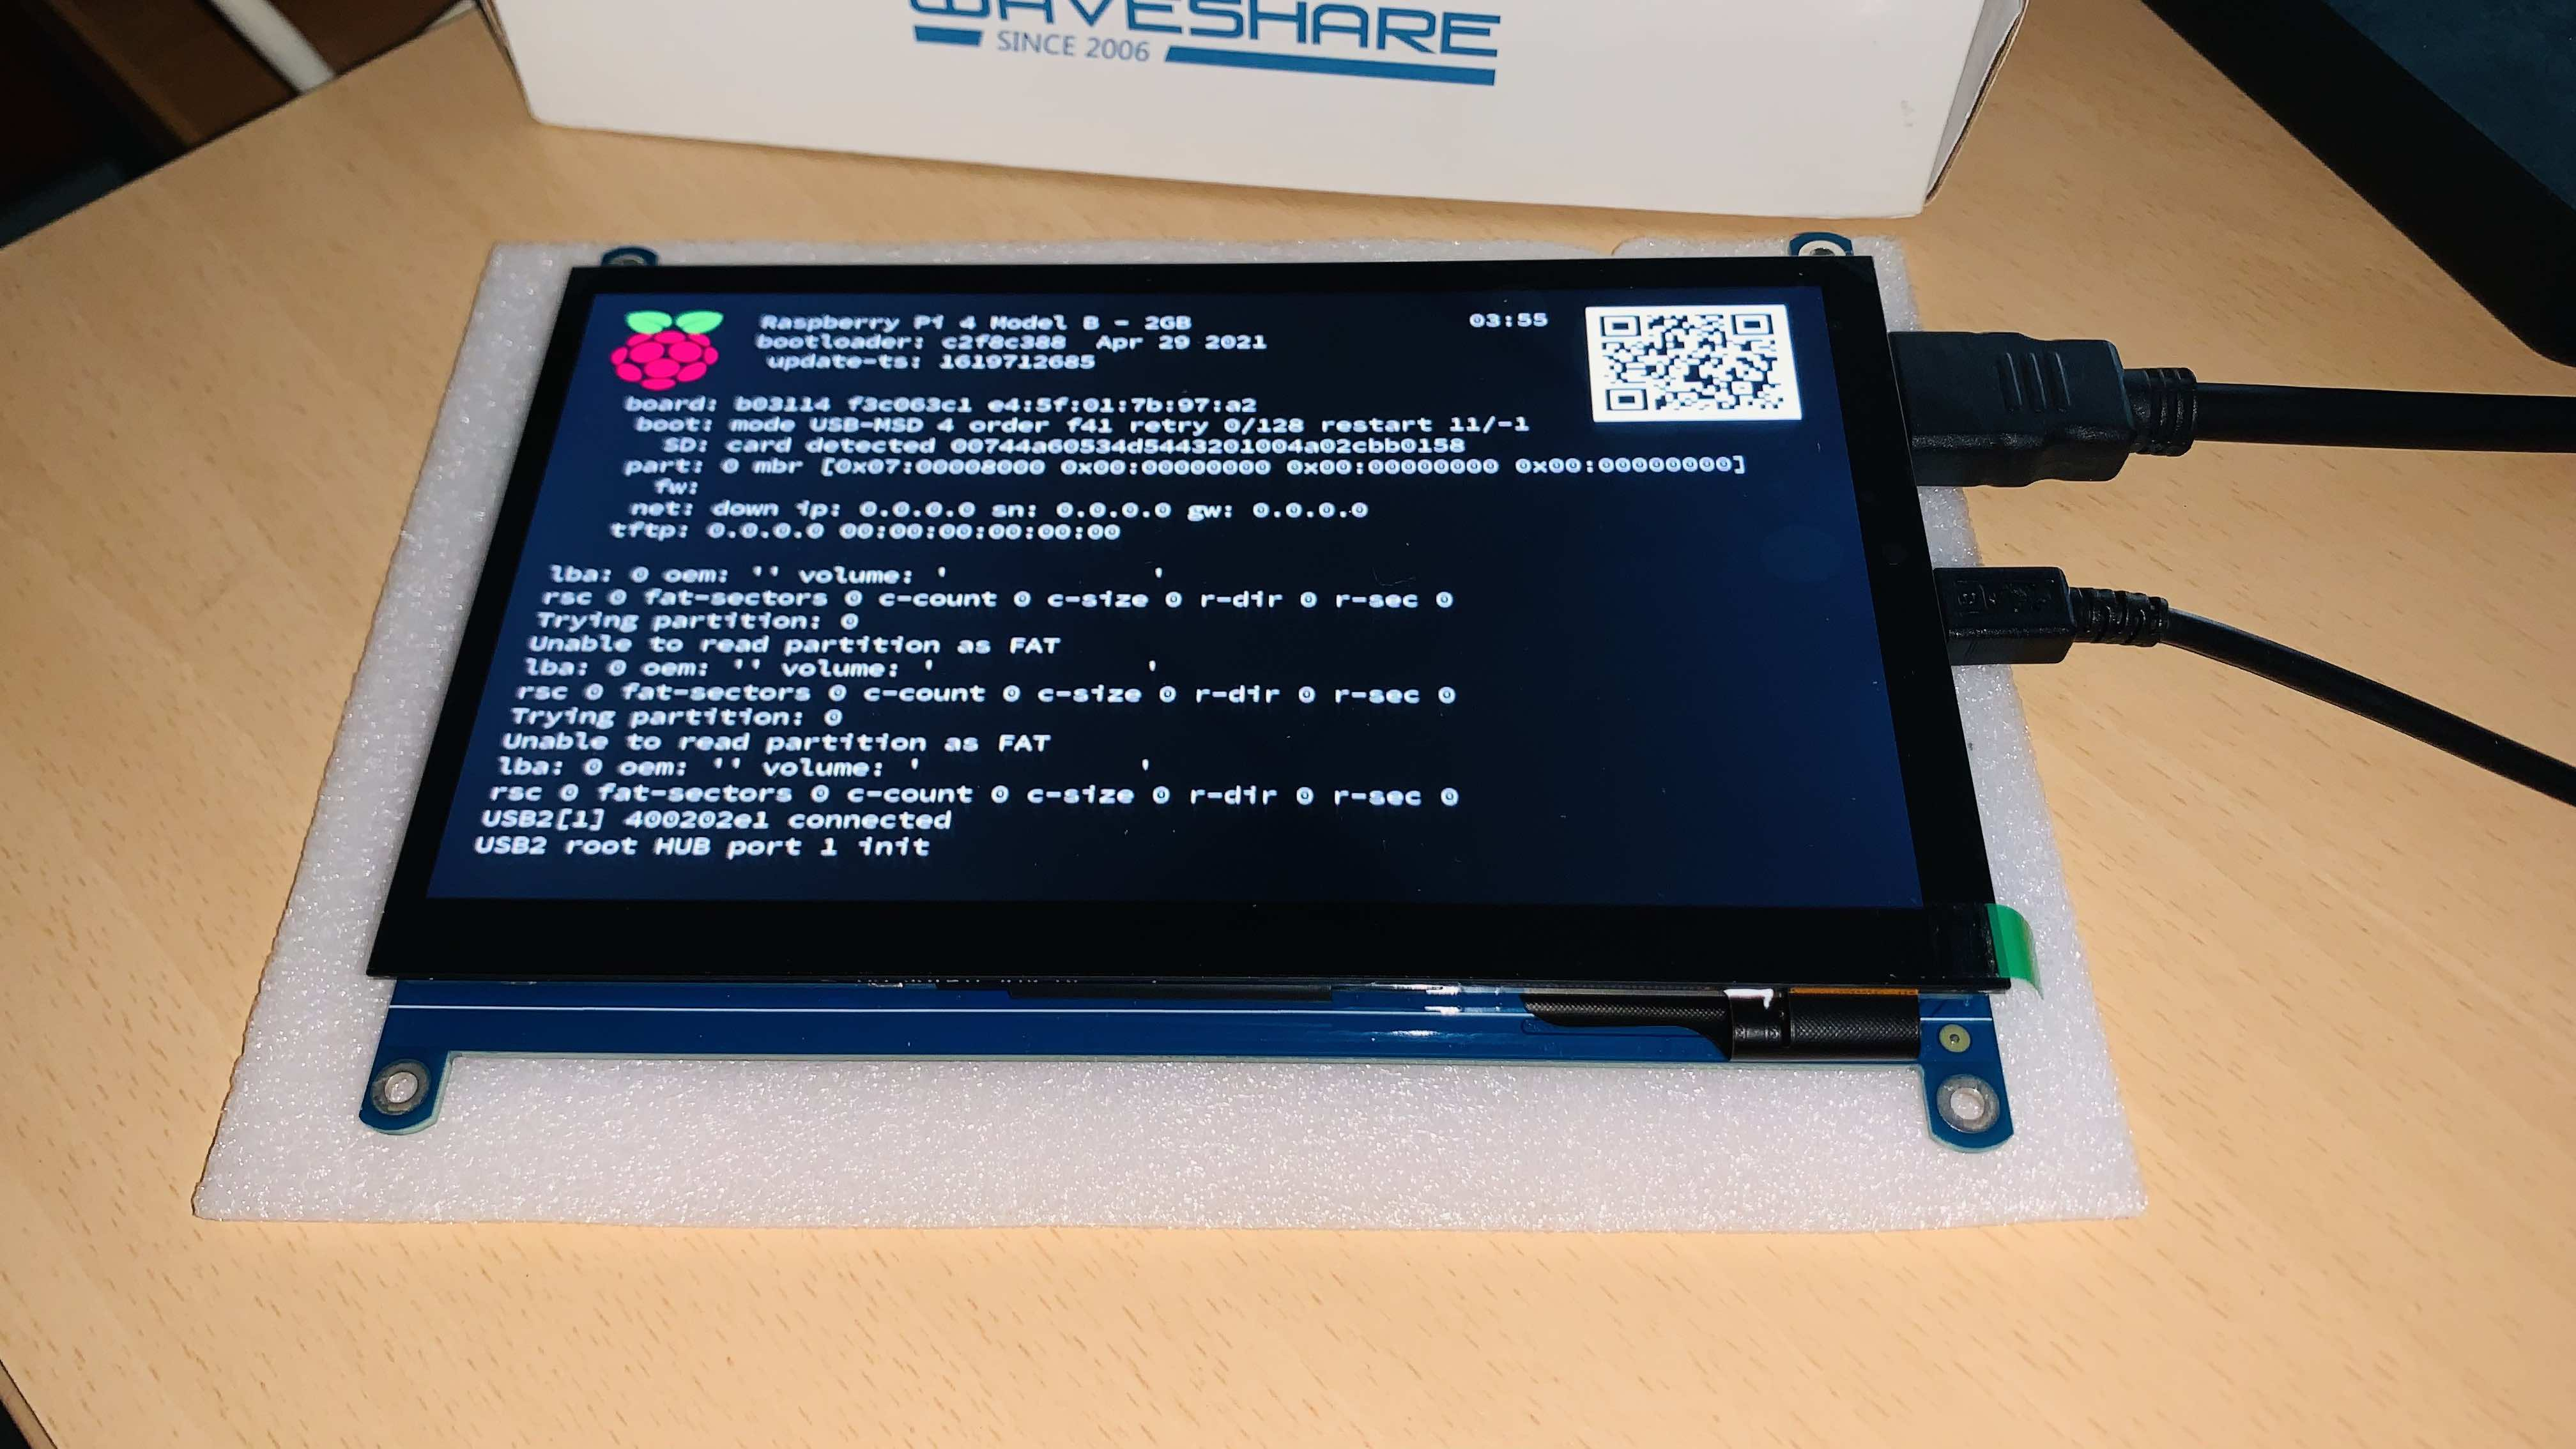
\includegraphics[scale=0.03]{raspberry_pi_lcd.jpeg} 
            \caption{Ecran LCD de 7 pouces}
        \end{figure}
    

    \section{Description, résultats attendus et objectifs}
    \section{Etude du besoin}
    \subsection{Contexte}
    \subsection{Analyse du besoin}
    \subsection{Définition des besoins}

    \section{Choix des technologies}
    \subsection{Choix du langage Python}
    \subsection{Choix l'API PiCamera}
    \subsection{Choix de la bibliothèque Tkinter}
    \section{Projet : Montage du dispositif de capture vidéo}

    \subsection{Objectifs}
        \begin{itemize}
            \item Montage du dispositif de capture vidéo
            \item Acquisition des données
            \item Traitement des données
            \item Visualisation des données
        \end{itemize}


    \section{Projet : Rélisation du logiciel de capture vidéo}
    \subsection{Objectifs}
        \begin{itemize}
            \item Réalisation du logiciel de capture vidéo
            \item Acquisition des données
            \item Traitement des données
            \item Visualisation des données
        \end{itemize}